%incorporating Ben's feedback
Aortic stenosis (AS) is a progressive degenerative valve condition that is the result of fibrotic and calcific changes to the heart valve. These structural changes occur over years and eventually lead to obstruction of blood flow, symptoms and death if not treated. AS is common and affects over 12.6 million adults and causes an estimated 102,700 deaths annually. AS can be effectively treated when it is identified in a timely manner though diagnosis remains challenging~\citep{yadgir2020global}. One promising route to improving AS detection is to consider automatic screening of patients at risk using cardiac ultrasound. Automatic screening could provide a systematic, reproducible process and augment current approaches that rely on cardiac auscultation and miss a significant number of cases~\citep{gardezi2018cardiac}.

% Aortic stenosis is an important valve disease.
% \todo{Explain it impacts million people over age 65}
% \todo{Explain it is easily treatable, but difficult to detect.}

% One promising route to improving detection of AS is to consider automatic screening of all routinely-collected transthoracic echocardiograms (TTEs). 
% Automatic screening could provide a systematic, reproducible process and augment current manual screening known to have inter-rater reliability issues.


\begin{figure}[!t]
\begin{tabular}{c c c}
\begin{minipage}{.45\textwidth}
(a) Human expert approach
\end{minipage}
& &
\begin{minipage}{.45\textwidth}
(b) Filter then Average {\scriptsize \citep{holste2022automated}}
\end{minipage}
\\
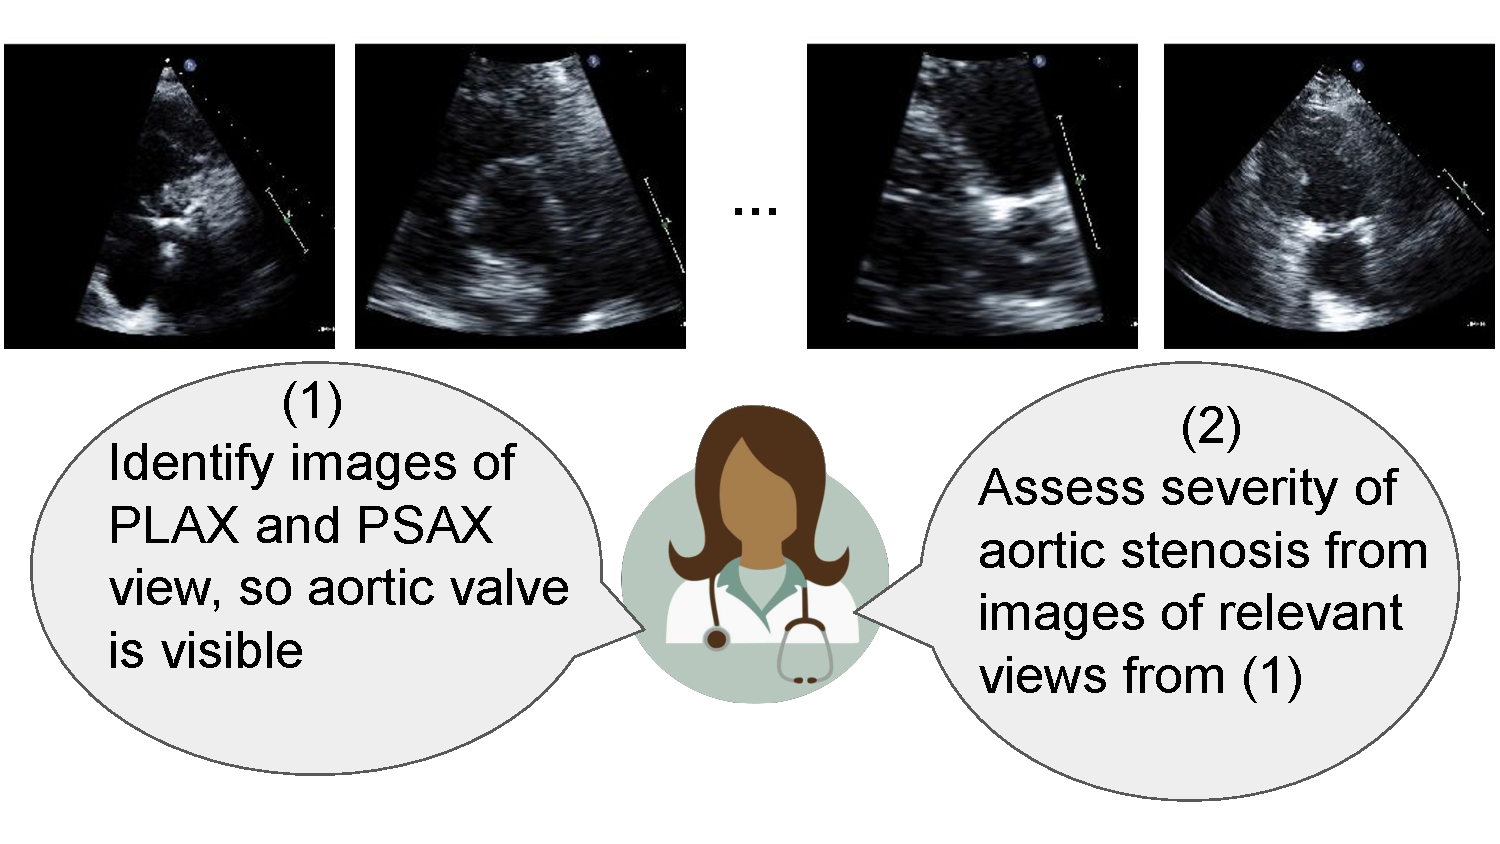
\includegraphics[width=0.45\textwidth]{figures/MIL_for_AS_diagram_1.pdf}
& &
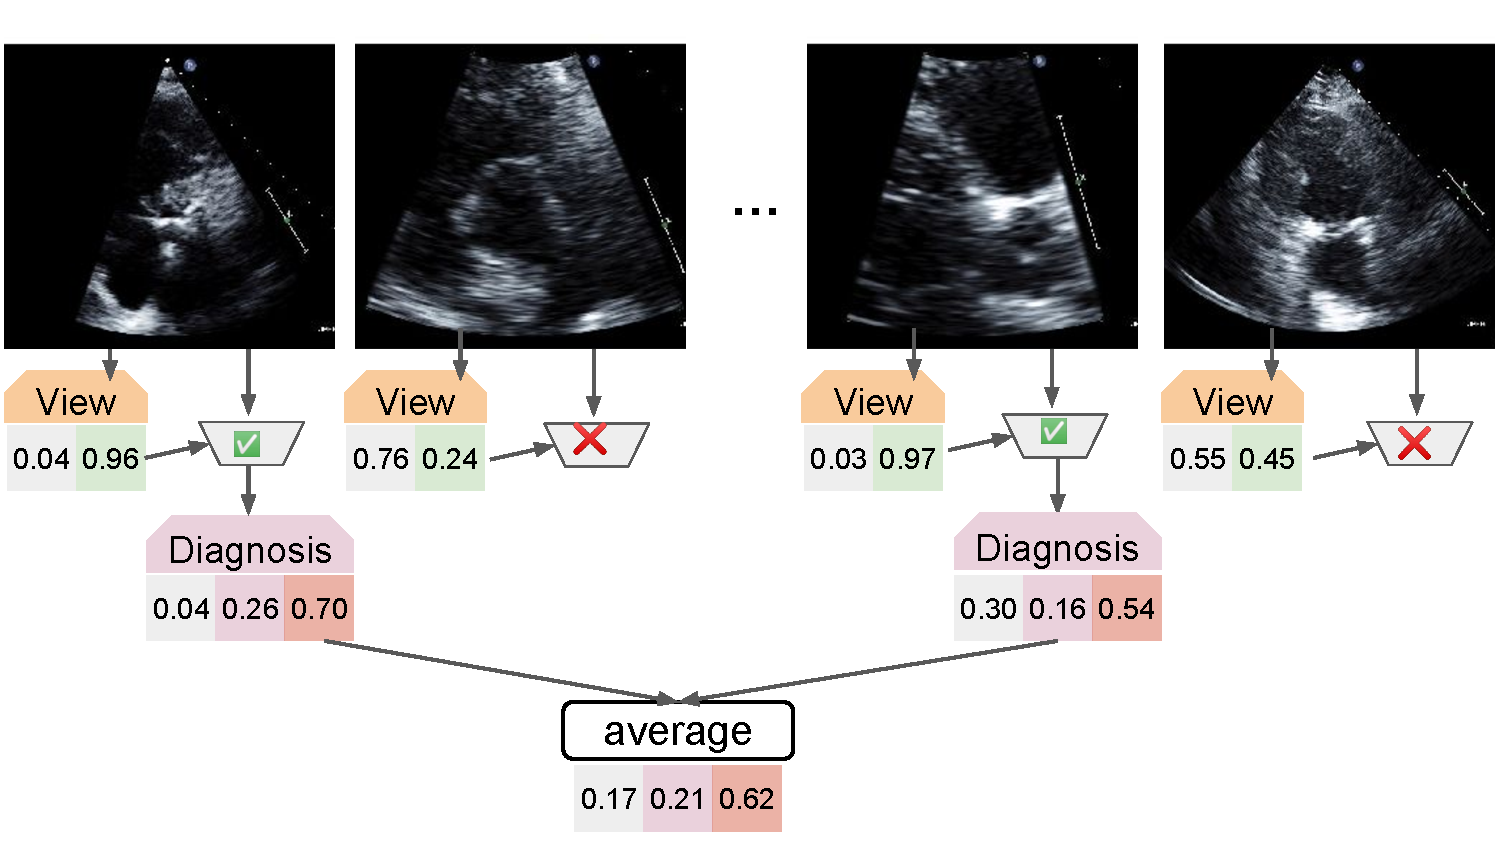
\includegraphics[width=0.45\textwidth]{figures/MIL_for_AS_diagram_2.pdf}
\\
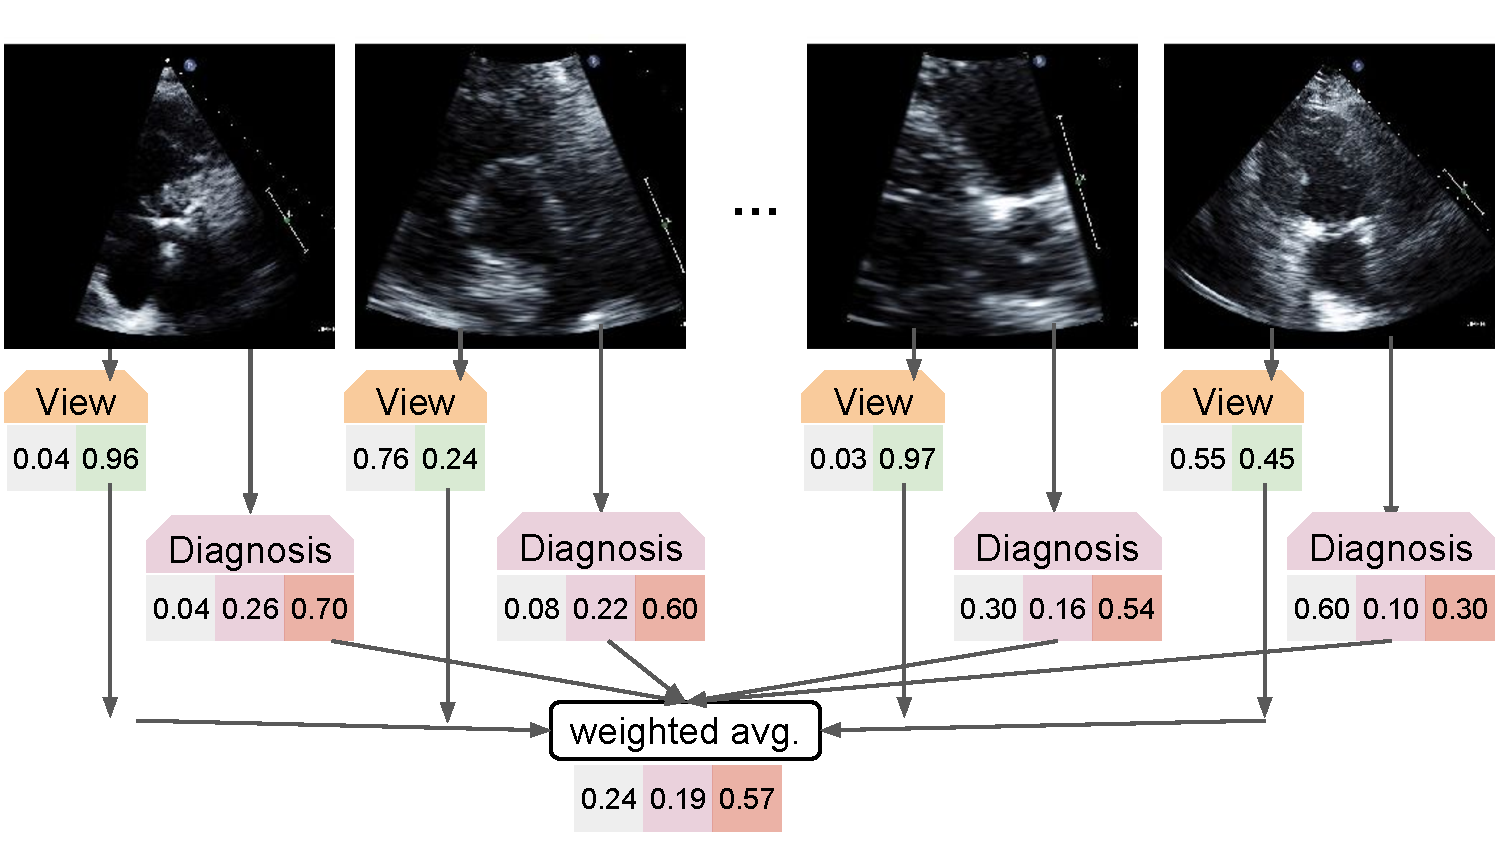
\includegraphics[width=0.45\textwidth]{figures/MIL_for_AS_diagram_3.pdf}
& &
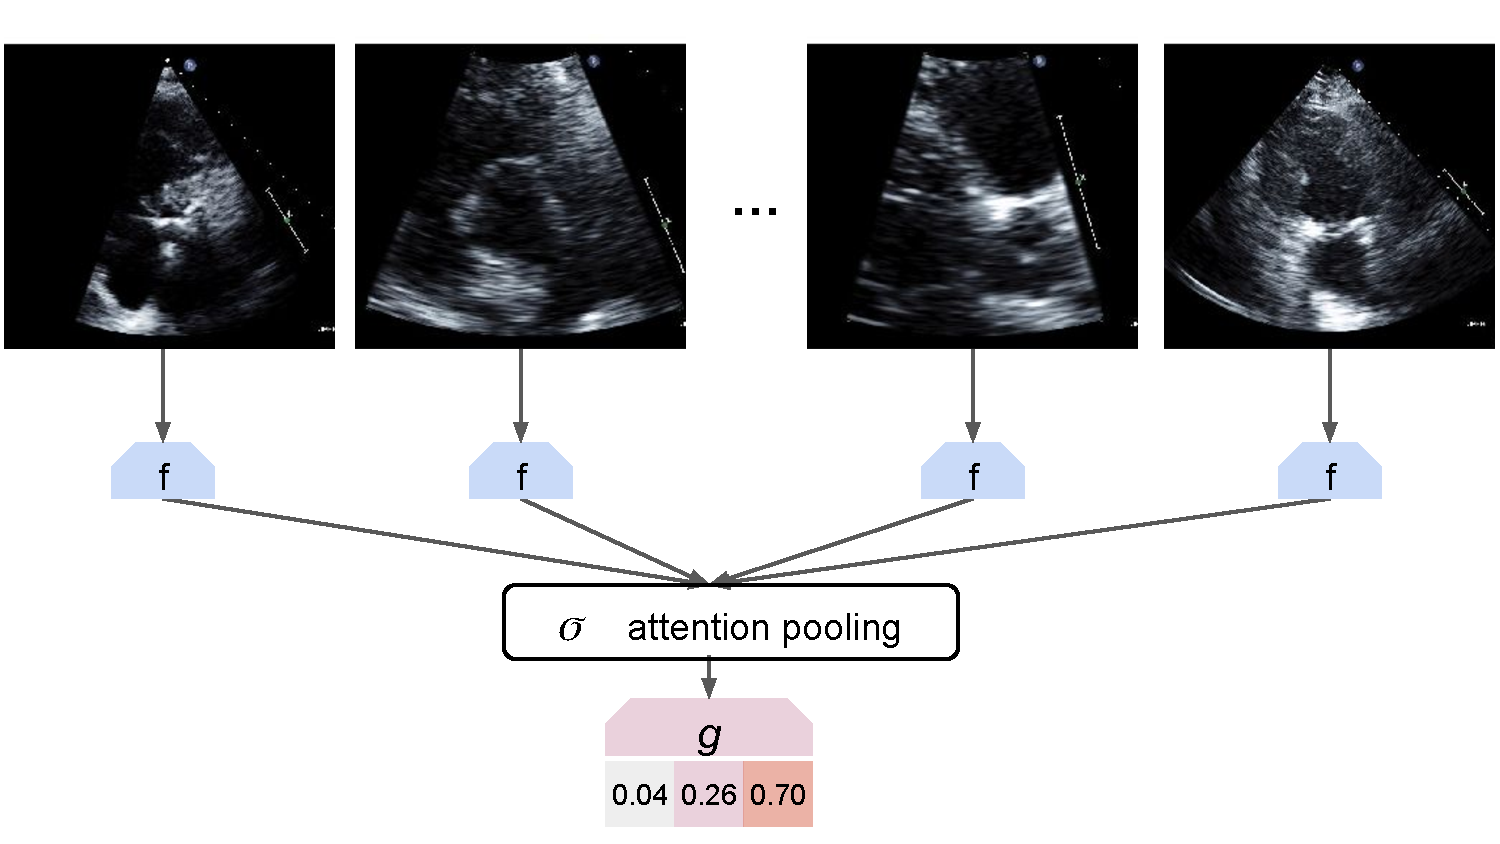
\includegraphics[width=0.45\textwidth]{figures/MIL_for_AS_diagram_4.pdf}
\\
\begin{minipage}{.45\textwidth}
(c) Weighted Average by View Relevance {\scriptsize \citep{wessler2023automated,huang2021new}}
\end{minipage}
& &
\begin{minipage}{.45\textwidth}
(d) Attention-based MIL ~\\
\end{minipage}
\end{tabular}
\caption{\textbf{Overview of methods for diagnosing aortic valve disease from multiple images of the heart.}
In our chosen diagnostic problem, the input is multiple ultrasound images representing different canonical view types of the heart's complex anatomy (e.g. PLAX, PSAX, A2C, A4C, and more, see \citet{mitchell2019guidelines} for a taxonomy).
The required output is a (probabilistic) prediction of the severity of Aortic Stenosis (AS), on a 3-level scale of no / early / significant disease.
We wish to develop deep learning methods that can solve this problem like expert cardiologists (panel a).
Two recent efforts (panel b by others, panel c by our group) made progress using a separately-trained view type classifier and per-image diagnosis classifier, but rely on combining diagnosis probabilities across images via average pooling that cannot learn how to distribute attention non-uniformly among images of relevant views.
In this work, we develop more flexible attention-based multiple instance learning architectures (MIL, panel d), with crucial contributions of supervised attention (Sec.~\ref{sec:methods_SA}) and improved pretraining strategies (Sec.~\ref{sec:methods_CL}) that we show later yield substantially improved performance on this task.
}%endcaption
\label{fig:diagrams}
\end{figure}

The challenge in developing a robust automated system for diagnosing AS is that echocardiogram studies consist of dozens of images or videos that show the heart’s complex anatomy from many different acquisition angles. As illustrated in Fig.~\ref{fig:diagrams} (a), clinical readers are trained to look across many images to identify those that show the aortic valve at sufficient quality and then use these “relevant” images to assess the valve’s health. Training an algorithm to mimic this expert human diagnostic process is difficult. Most standard deep learning classifiers are designed to consume only one image and produce one prediction. Automatic screening of echocardiograms requires the ability to make one coherent prediction from \emph{many} images representing diverse view types. To make matters more difficult, each image’s view type is not recorded in the EHR during routine collection.

% The challenge is that an echocardiogram study consists of dozens of images or videos that show the heart's complex anatomy from many different acquisition angles.
% Clinical readers are trained to look across many images to identify those that show the aortic valve at sufficient quality and then use these ``relevant'' images to assess the valve's health. Training an algorithm to mimic this expert human diagnostic process is difficult.
% Most standard deep learning classifiers are designed to consume only one image and produce one prediction. Automatic screening of echocardiograms requires the ability to process \emph{many} images representing diverse view types. Each image's view type is not stored in the EHR during routine collection.

Multiple-instance learning (MIL) is a branch of weakly supervised learning in which classifiers can consume a variable-sized set of images to make one prediction.
Recent impressive advances in MIL have been published ~\citep{ilse2018attention, lee2019set, sharma2021cluster, shao2021transmil}. 
However, their success on ultrasound tasks, especially those with images from many possible view types, has not been carefully evaluated.

% Our approach does not require the separately-trained filtering step (Fig.~\ref{fig:diagrams} (b)) for selecting relevant views for diagnosis needed by some previous AS screening methods~\citep{holste2022automated}.
\subsection*{Contributions to clinical translation and MIL methodology}
This study's contribution to applied clinical research is the development and validation of a new deep MIL approach for automatic diagnosis of heart valve disease from multiple ultrasound images produced by a  routine trans-thoracic echocardiogram (TTE) study. 
Our end-to-end approach can take as input any number of images from various view types. Our approach eliminates the need for a separately-trained filtering step (Fig.~\ref{fig:diagrams} (b)) to select relevant views for diagnosis, as required by some prior AS screening methods ~\citep{holste2022automated}. Our approach is also more flexible and data-driven than the weighted average (Fig.~\ref{fig:diagrams} (c)) of other previous efforts of AS screening~\citep{huang2021new,wessler2023automated}.
Head-to-head evaluation in Sec.~\ref{sec:Results} demonstrates that our approach can yield superior balanced accuracy for assigning AS severity grades to new studies, while keeping model size over 4x smaller than previous efforts like \citep{holste2022automated}.
Small model sizes enable faster predictions and ease portability to new hospital systems.

Our approach's success is made possible by two methodological contributions. % MIL research. 
First, we propose a supervised attention mechanism (Sec.~\ref{sec:methods_SA}) that steers focus toward images of relevant views, mimicking a human expert.
On our AS diagnosis task, supervised attention yields notable gains -- balanced accuracy jumps from 60\% to over 70\% -- over previous off-the-shelf attention-based MIL~\citep{ilse2018attention}.
Second, we introduce a self-supervised pretraining strategy (Sec.~\ref{sec:methods_CL}) that focuses contrastive learning on the embedding of an entire study (a.k.a. the embedding of the ``bag'', using MIL vocabulary). In contrast, most previous pretraining focuses on representations of individual images.
Both innovations are broadly applicable to other MIL problems involving imaging data of multiple view types.
%we introduce a novel self-supervised pretraining strategy that contrasts the bag-level embedding instead of image-level embedding, which are shown to be more effective for our problem (might also be suitable for other MIL problem).

%This study makes three contributions towards the automatic diagnosis of Aortic Stenosis using machine learning. Firstly, we propose an end-to-end multi-instance-learning approach that can diagnose Aortic Stenosis in realistic clinical scenarios, consuming various numbers of images from different view types in a realistic TTE study, without requiring pre-filtering. Secondly, we leverage clinical insights and introduce a supervised attention mechanism that uses predicted view relevance to guide the model's attention, significantly improving the performance of off-the-shelf MIL algorithms. Thirdly, we propose a novel self-supervised pre-training strategy that contrasts the bag-level embeddings, instead of the image-level embeddings, which we demonstrate to be more effective for our problem and may also be suitable for other MIL problems.

\subsection*{Generalizable Insights about Machine Learning in the Context of Healthcare}

This study offers critical insight into how multiple-instance learning can be applied to routine echocardiography studies. We show that recent MIL architectures are insufficient in achieving competitive performance and lack the ability to make \textbf{clinically plausible} decision (they attends to irrelevant instances). Our two innovations -- supervised attention (Sec. \ref{sec:methods_SA}) and bag-level self-supervised pretraining (Sec.~\ref{sec:methods_CL}.) can be broadly applicable to many clinical image analysis problems that require non-trivial aggregation over multiple images from multiple acquisition angles (views) to make one diagnosis. Beyond echocardiography, these insights could be useful for lung ultrasound, fetal ultrasound, head CT, and more.
%all of which require the clinical expert to aggregate information across multiple images from multiple acquisition angles (views).
